\documentclass[a4paper,spanish] {article} 
\usepackage [spanish] {babel} 
\usepackage [latin1]{inputenc}
\usepackage{graphicx}
\usepackage{caratula}
\usepackage{subfig}
\usepackage{dsfont}
\usepackage{algorithm}
\usepackage{amsmath}
\usepackage{algorithmic}


\addtolength{\oddsidemargin}{-1in}
\addtolength{\textwidth}{2in}

\begin{document}
\pagestyle{headings}



\newpage

\materia{Aprendizaje por Refuerzos: Teor\'ia y Aplicaciones en Rob\'otica, Psicolog\'ia y Neurociencias}
\submateria{Tp Final}
\titulo{Desarrollo de algoritmos de aprendizaje y an\'alisis de resultados en una adaptaci\'on del problema Bomberman}

\integrante{Pablo Brusco}{527/08}{pablo.brusco@gmail.com}
\integrante{Carolina Hadad}{367/08}{carolinahadad@gmail.com}
\integrante{Sergio Medina}{216/05}{medinasergio@gmail.com}
\integrante{Santiago Palladino}{138/05}{spalladino@gmail.com}
\integrante{Andres Taraciuk}{228/05}{ataraciuk@gmail.com}


\maketitle

		
\newpage
\tableofcontents
\newpage

\section{Objetivo}
	En  este Trabajo Practico nos interesa analizar el desempe\~ no de los algoritmos de aprendizaje vistos durante el curso,  aplic\'andolos  en un problema distinto de los planteados en las clases. En nuestro caso, elegimos adaptar el juego del Bomberman. 
	
	Compararemos los resultados del aprendizaje en agentes tanto model-free como model-based, con los algoritmos de QLearning, RMax, Sarsa, Sarsa Lambda, y Dyna mostrando cu\'ales de ellos funcionan mejor en nuestro caso. Intentaremos explicar tambi\'en a qu\'e se deben estos resultados. Adem\'as analizaremos el efecto de aplicar rewards intermedios en el tiempo de aprendizaje del agente y c\'omo var\'ia el aprendizaje del agente al moverse en un ambiente estoc\'astico con distintas condiciones de aleatoriedad.

\section{Introducci\'on}
	\subsection{Adaptaci\'on del juego del Bomberman}
	El juego que vamos usar es una versi\'on simplificada del juego del Bomberman. El objetivo del agente es llegar a la salida. El agente tiene 4 acciones de movimiento: arriba, abajo, hacia la izquierda y hacia la derecha. El tablero tiene paredes que obstaculizan su camino, algunas de ellas son rompibles y otras irrompibles. El agente tiene acciones para poner una bomba y para explotarla. Solo puede haber una bomba en el tablero, por lo que si el agente realiza una acci\'on de tirar bomba habiendo una bomba en el juego, la acci\'on no tendr\'a efecto. Al explotar la bomba se destruir\'an las paredes que est\'en arriba, abajo a la izquierda y a la derecha de ella. Si el agente estuviera en alguno de estos lugares o sobre la bomba, el agente morir\'ia, teniendo que empezar el juego nuevamente desde la posici\'on inicial. 
	
	Nos interesa que el agente aprenda una pol\'itica para llegar a la salida realizando la menor cantidad de acciones posibles, para esto le damos un refuerzo positivo grande en el momento que llega al casillero de salida y un refuerzo negativo de la misma magnitud cuando el agente muere. A estos refuerzos los llamaremos \texttt{WIN\_REWARD} y \texttt{LOSE\_REWARD} respectivamente.
	
\section{Representaci�n del estado}

	En nuestro programa vamos a representar el Estado como una tupla con los valores que listaremos a continuaci\'on:
\begin{itemize}
\item \textbf{bomberman position}: Tupla con la posici�n $i,j$ del agente en el tablero, en un momento determinado; valor inicial $(0,0)$.
\item \textbf{bomb position}: Tupla con la posicion $i,j$ de la bomba en el tablero, si es que la hay; toma un valor distinguido en caso de que no haya una bomba presente.
\item \textbf{stones}: Arreglo de valores booleanos. Cada posici�n $i$ del arreglo indica si esa pared rompible est� presente en el tablero, es decir si a\'un no fue destruida por el agente. El orden de las paredes va de arriba a la izquierda a abajo a la izquierda. Inicialmente est�n todas presentes. En el archivo \textit{sample\_board.txt} se puede ver la configuraci�n de los distintos tableros usados.
\item \textbf{died}: Valor booleano que indica si el agente muri�, lo que implica el fin de la partida.
\end{itemize}

Mediante esos valores podemos identificar un\'ivocamente cada configuraci\'on posible del juego. Por cuestiones de consumo de memoria, para los algoritmos no factorizados, optamos por seguir el mecanismo usual de traducir cada estado en un entero \'unico que lo representa. En todas las estructuras de datos utilizadas en los distintos agentes, el valor almacenado es simplemente num\'erico, lo que hace que el agente sea completamente agn\'ostico de la conformaci\'on del estado.

Para el caso del agente RMax Factorizado, que requiere que el estado se encuentre segmentado en factores, optamos por proveer una funci\'on que identifique con un entero de manera \'unica los posibles valores de cada uno de los factores individualmente.

Asimismo, a\'nadimos un quinto factor redundante para el uso con RMax Factorizado:
\begin{itemize}
\item \textbf{delta bomb}: Tupla $\Delta i, \Delta j$ que indica la distancia (en valor absoluto) del agente a la bomba lanzada, si la hubiera.
\end{itemize}

Si bien este \'ultimo factor puede inferirse directamente a partir de bomberman position y bomb position, como veremos m\'as adelante, nos permite vincular en la DBN la muerte del bomberman solamente con su posici\'on relativa a la bomba; de esta manera esperamos que el agente aprenda el concepto de que muere si explota al lado de una bomba, en lugar de que aprenda en qu\'e casos muere para todas las combinaciones de su posici\'on y de la bomba en el tablero.

La implementaci\'on de la clase estado, su factorizaci\'on y las funciones de conversi\'on a enteros puede verse en el archivo \textit{state.py}.

\section{Acciones posibles del agente}

	El agente cuenta con 4 acciones de movimiento: \texttt{UP}, \texttt{DOWN}, \texttt{LEFT} y \texttt{RIGHT}. Estas acciones, cambian su posici�n en el tablero. Adem�s puede lanzar una bomba (s�lo una por vez, no puede haber 2 bombas activas en el juego) con la acci�n \texttt{DROP\_BOMB}. La bomba es ubicada en la posici�n en la que estaba el agente cuando la la bomba fue lanzada. El agente puede, por �ltimo, explotar la bomba mediante la acci�n \texttt{EXPLODE}. El radio de alcance de la bomba es de el casillero donde esta ubicada la bomba y sus aleda�os, es decir el de arriba, el de abajo, el de la izquierda y el de la derecha. Cuando una bomba explota destruye las paredes rompibles (\texttt{STONES}) que est�n en su radio de alcance y mata al agente si este se encuentra en este radio. Una vez que la bomba es explotada, el agente puede lanzar otra.
	
	Esta informaci�n se puede ver en la clase $Action.py$.



\section{Uso}
	Para correr el programa se debe elegir una configuraci�n para los par\'ametos en alg\'un archivo de la carpeta settings. Luego, agregar el nombre del archivo modificado en la lista de \texttt{RUN\_CONFIGURATIONS} del archivo Runner.py. Luego, basta ejecutar el archivo \textit{Runner.py} y se correr\'an todas las configuraciones agregadas a la lista de \texttt{RUN\_CONFIGURATIONS}.
	
	Los archivos de settings deben tener valores para los siguientes par\'ametros:
\begin{enumerate}
\item \texttt{CONFIGURATION\_NAME}
\item \texttt{ITERATIONS}: cantidad de veces que correr� el algoritmo. El algoritmo corre hasta que el agente muere, llega a la salida o llega a la m\'axima cantidad de acciones posible.
\item \texttt{MAX\_TURNS}: M\'axima cantidad de acciones que puede realizar el agente hasta que el juego se de por terminado.
\item \texttt{AGENT}: algoritmo de aprendizaje del agente que correr\'a. Se pueden elegir los siguientes algoritmos:
\begin{itemize}
\item \texttt{QLEARNING}
\item \texttt{RMAX}
\item \texttt{FACTOREDRMAX}
\item \texttt{SARSA}
\item \texttt{SARSALAMBDA}
\item \texttt{DYNA}
\end{itemize}
	
\item \texttt{TASK}: determina el tipo de ambiente en el que correr\'a el agente. El agente puede correr en un ambiente determin\'istico o estoc\'astico. En los ambientes estoc\'asticos, con cierta probabilidad, las acciones no tienen el efecto esperado. Desarrollamos las siguientes opciones para este par\'ametro:
\begin{itemize}
\item \texttt{DETERMINISTIC}: cada acci�n causa el mismo resultado siempre.
\item \texttt{STOCHASTIC\_NAVIGATION}: con cierta probabilidad, las acciones de movimiento causan que el agente se mueva en otra direcci\'on. Por ejemplo podria pasar que algente realice la acci\'on UP y que el efecto sea el mismo que el que hubiera causado realizar la acci\'on LEFT en un ambiente deterministico, por ejmplo.
\item \texttt{STOCHASTIC\_EXPLOSION}: Con cierta probabilidad la acci\'on de explotar bomba no la detona. La bomba queda en el mismo lugar en donde el agente la puso. Esto simula el caso en el que el detonador a veces no funciona.
\end{itemize} 
	De todas maneras explicaremos m�s sobre esto en la secci�n $Ambiente \ Estocastico$ 

\item \texttt{IS\_IMMORTAL}: si este booleano esta en True, el agente no muere al detonarse una bomba, pese a estar ubicado en su rango de explosi�n.
\item \texttt{MAP\_SIZE}: El tama�o del mapa. Se puede elegir entre mapas de tama�o 3, 5 u 8. Las distribuciones de walls y stones (paredes irrompibles y rompibles) para cada uno de estos mapas, se puede ver en el archivo sample\_board.txt.
\item \texttt{BOMB\_EXPLODING\_PROBABILITY}: La posibilidad de que las bombas exploten.
\item \texttt{BOMB\_REWARD\_POLICY}: Pol�tica de refuerzo intermedio por explotaci\'on de bomba. M\'as adelante en el informe explicaremos cuales son las opciones posibles y qu\'e significa cada una.
\item \texttt{NAVIGATION\_REWARD}: Pol�tica de refuerzo intermedio por posici\'on del agente. Tambi\'en explicaremos mas adelante cu\'ales son las opciones para este par\'ametro.
\item \texttt{WIN\_REWARD}: Refuerzo por llegar a la salida.
\item \texttt{LOSE\_REWARD}:Refuerzo negativo por morir.
\item \texttt{BOMB\_REWARD}:Refuerzo intermedio por explotar bomba que se usa de acuerdo a la pol\'itica de refuerzos intermedios adoptada.
\item \texttt{NO\_ACTION\_NEGATIVE\_REWARD}: Si este flag est\'a activado se le da un refuerzo negativo al agente cada vez que realiza una acci\'on que no cambia el estado
\item \texttt{INITIAL\_REWARD}: Refuerzo por acci�n realizada. Puede estar en 0 o tener un valor negativo.
\item \texttt{USE\_DELTABOMB\_FACTOR}: Booleano que si est\'a en True indica que se debe agregar al estado una tupla con la posici�n del bomberman respecto de la bomba lanzada. Se usa para Rmax y ser\'a explicado m\'as adelante.
\end{enumerate}
	

\section{Visualizaci\'on}


\section{Arquitectura}
	%pagina http://yuml.me/diagram/scruffy/class/draw
	%codigo [Manager| run()]->1[Task|start(); perform(action)]
	%		[Task] ->1[Environment|start(); performAction(action)]
	%		[Manager]->1[Agent | learn(); nextAction()]
	
	Las clases mas importantes de la arquitectura son: Agent, Task, Environment y Manager.
	
	Como lo indica el modelo conceptual que se muestra debajo, el Manager es la clase que hace interactuar a la Task (y por medio de esta, al Environment) con el Agent. La responsabilidad del Manager es bastante simple: corre un ciclo en el cual ejecuta acciones en la Task, le da la informaci\'on requerida al Agent para que aprenda y luego le indique la pr�xima acci\'on a tomar.
	El Environment es el encargado de ejecutar acciones en el juego del Bomberman y de mantener su estado, el mismo es agnostico de refuerzos, de los cuales se encarga la Task (la cual es tambi\'en la encargada de implementar aleatoriedad, que se explicar\'a luego).
	
	
	\begin{figure}[h!]
  \centering
    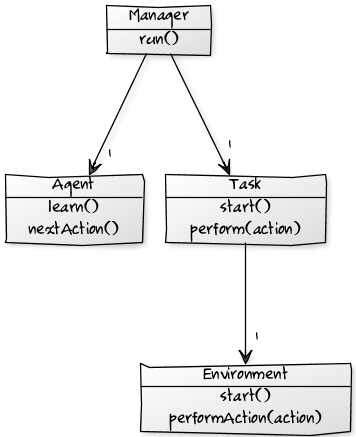
\includegraphics[width=0.5\textwidth]{MCarquitectra.png}
  \caption{Modelo Conceptual de la Arquitectura.}

	\end{figure}
\section{Algoritmos de Aprendizaje}
	Programamos agentes con pol\'iticas de aprendizaje distintas. En esta secci�n explicaremos en detalle qu� agentes hicimos, c�mo implementamos cada una de las pol�ticas de aprendizaje y algunas caracter�sticas te�ricas de los algoritmos implementados. 
	\subsection{Agentes Model-Free}
		\newpage
			\clearpage
	\subsubsection{QLearning}
	
\paragraph{}	Q-learning es una t�cninca que funciona aprendiendo una funci�n en base a acciones-valores que devuelve el refuerzo esperado por tomar la acci�n dada en un estado dado y siguiendo una pol�tica fija. Lo importante es que no requiere aprender el modelo del problema.
	
	
\paragraph{}El modelo del problema consiste en un agente, estados S, y un n�mero de acciones por estado A. Realizando las acci�nes , el agente puede moverse de estado a estado. Cada estado provee al agente de una recompenza (un n�mero natural en nuestro caso) o castigo (una recompenza negativa). El objetivo del agente es maximizar la recompenza total. Lo cual logra aprendiendo que acci�n es optima para cada estado.

\paragraph{}El algoritmo, por lo tanto, posee una funci�n que calcula la calidad de un par estado-acci�n.

$Q: S \times A \leftarrow \Re$

\paragraph{}Antes que el aprendizaje empiece, la funci�n Q retorna un valor fijo, elegido por el dise�ador del algoritmo. Luego, cada vez que el agente recibe una recompenza, nuevos valores son calculados para cada combinaci�n de estado-acci�n de S x A. El nucleo del algoritmo es una simple actualzaci�n iterada de valores, la cual actualiza los valores en base a nueva informaci�n.


$$Q(s_t,a_t) \leftarrow \underbrace{Q(s_t,a_t)}_{\footnotesize{\textrm{ viejo valor}}} + \underbrace{\alpha}_{\footnotesize{\textrm{tasa aprendizaje}}}*\left[ \overbrace{ \underbrace{r_{t+1}}_{\footnotesize{\textrm{ recompenza}}} + \underbrace{\gamma}_{\footnotesize{\textrm{factor de descuento}}}* \underbrace{\max_aQ(s_{t+1},a)}_{\footnotesize{\textrm{m�ximo valor futuro}}}}^{\footnotesize{\textrm{recompenza descontada esperada}}} - \underbrace{Q(s_t,a_t)}_{\footnotesize{\textrm{ viejo valor}}}\right]  $$


Un episodio del algoritmo termina cuando el estado $s_{t+1}$ es un estado final.


\paragraph{ Influencia de las varibles en el algoritmo.}

\paragraph{}\textbf{$\alpha$ (Learning rate)}\\
 La tasa de aprendizaje es el que determina que importancia darle a la nueva informaci�n, un factor cerca de 0 implica que el agente aprenda muy poco y una tasa cerca de 1 implica que el agente considerar� mayormente la informaci�n reciente.

\paragraph{}\textbf{$\delta$ (Discount factor)}\\
 El factor de descuento determina la importancia de futuras recompenzas. Un factor cerca de cero har� que el agente concidere solo su acci�n en el momento y no sus consecuencias futuras, contrario al caso de un factor cerca de uno donde el agente conciderara las recompenzas a largo plazo. (si el factor es mayor a uno Qleaning diverge)

\paragraph{Implementaci�n:}

Q learning usa una tabla para almacenar los datos obtenidos, en nuestro caso un simple diccionario con claves (acci�n,estado) y el valor de la funci�n Q como valor. A continuaci�n, veremos el pseudoc�digo utilizado:

	\clearpage
		\begin{figure}[h!]
			\centering
			\includegraphics[width=0.5\textwidth]{qLearning.png}
			\caption{Algoritmo QLearning}
		\end{figure}
	
	
	\subsubsection{Sarsa}

		\begin{figure}[h!]
		\centering
		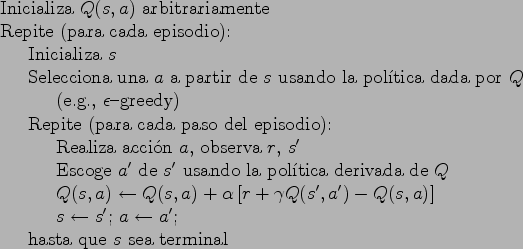
\includegraphics[width=0.5\textwidth]{Sarsa.png}
		\caption{Algoritmo Sarsa}
		\end{figure}
	
	
	\subsubsection{Sarsa ($\lambda$)}	

		\begin{figure}[h!]
			\centering
			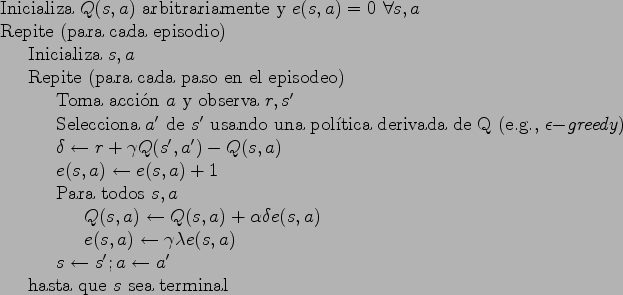
\includegraphics[width=0.5\textwidth]{SarsaLambda.png}
			\caption{Algoritmo Sarsa ($\lambda$)}

		\end{figure}
	
	\subsubsection{Dyna-Q}
		
		\begin{figure}[h!]
			\centering
			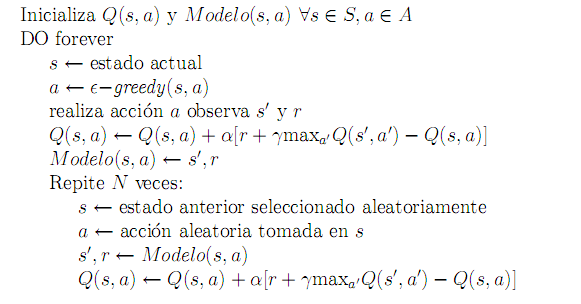
\includegraphics[width=0.5\textwidth]{Dyna.png}
			\caption{Algoritmo Dyna-Q}
		\end{figure}
	
	
	\subsection{Agentes Model-Based}	
		\subsubsection{RMax}

Para implementar Rmax en nuestro trabajo, decidimos basarnos en la versi�n de KWIK-Rmax presente en las slides de la quinta clase del curso. Adem�s, para m�s detalle sobre KWIK, y sobre las cotas matem�ticas necesarias, nos basamos fuertemente en una disertaci�n de Lihong Li \cite{li}.

Un agente Rmax, al ser model based, va armando un modelo completo en base a la experiencia adquirida y, al momento de decidir qu� acci�n tomar, elige aqu�lla que considera m�s valiosa en base a todo el modelo que tiene computado el agente. Entonces, el algoritmo se divide en dos fases: una fase de aprendizaje, donde actualizamos el modelo en base a la experiencia emp�rica, y la fase de toma de decisi�n, donde, en base al modelo, mediante alguna t�cnica como value iteration, decidimos qu� acci�n es la que m�s conviene tomar.

Al usar una versi�n KWIK para Rmax con las cotas necesarias, se garantizar�a que el algoritmo completo fuera PAC. 

\subsubsection{RMax Factorizado}

\section{Ambiente Estocastico}

	Se implementaron dos versiones que agregan aleatoriedad al juego, en relaci\'on a la navegaci\'on y a la explosi\'on de las bombas.\\
	
	\textbf{Navegaci\'on}: Cuando el Bomberman intenta realizar una acci\'on de navegaci\'on, puede que la misma se ejecute (con una cierta probabilidad) o alguna de otras dos opciones. Estos par\'ametros son configurables pero la configuraci\'on por defecto es la siguiente:
	
\begin{center}
\begin{tabular}{ l | c | r }
  Acci\'on Ejecutada & Opci\'on 1 & Opci\'on 2 \\
  \hline
  Arriba (80\%) & Izquierda (10\%) & Derecha (10\%) \\
  Abajo (80\%) & Izquierda (10\%) & Derecha (10\%) \\
  Izquierda (80\%) & Arriba (10\%) & Abajo (10\%) \\
  Derecha (80\%) & Arriba (10\%) & Abajo (10\%) \\  
\end{tabular}
\end{center}

	La clase encargada de implementar esto es StochasticNavigationTask y se configura seteando como \texttt{TASK} el valor \texttt{STOCHASTIC\_NAVIGATION}.\\
	
		\textbf{Explosi\'on}: Cuando el Bomberman intenta explotar una bomba, esta puede explotar o no con cierta probabilidad. Si bien los par\'ametros son configurables la probabilidad de explosi\'on por defecto es 80\%. Se configura seteando como \texttt{TASK} el valor \texttt{STOCHASTIC\_EXPLOSION}.
	
 \section{Pol\'iticas de Refuerzo}
 	Para evaluar el efecto de aplicar pol\'iticas de refuerzos intermedios en el tiempo de aprendizaje de los agentes, incluimos los siguientes campos en el archivo de settings, que se agregan al refuerzo por llegar a la salida y al refuerzo negativo en el caso de que el agente muera. En el caso de que el agente llegue a la salida o muera recibe el \texttt{WIN\_REWARD} o el \texttt{LOSE\_REWARD} respectivamente, y no se agrega este refuerzo adicional.

\begin{description}
\item[\texttt{NAVIGATION\_REWARD}] Rewards por posici\'on del agente.
	\begin{itemize}
	\item \texttt{NAVIGATION\_NO\_REWARD}: No se agrega refuerzos intermedios adicionales.
	\item \texttt{NAVIGATION\_REWARD\_PROPORTIONAL\_TO\_EXIT}: Siempre que el agente realice una acci\'on que cambie su posici\'on recibe un refuerzo adicional proporcional a su distancia a la salida. En el caso de las acciones de movimiento que no cambien el estado, como por ejemplo intentar moverse hacia una posici\'on que tenga una pared, el agente no recibir\'a ning\'un refuerzo, de manera de desalentar este tipo de acciones. 
	
	Las formula para el c\'alculo de este refuerzo intermedio es la que sigue:
	$$ refuerzo = cercania\_en\_x + cercania\_en\_y $$
	donde
	$$ cercania\_en\_x =\mid map\_size-1 -(exit_0 - agentPosition_0) \mid$$
	$$ cercania\_en\_y =\mid map\_size-1 -(exit_1 - agentPosition_1) \mid$$
	siendo $exit = (exit_0, exit_1)$ la posici\'on de la salida en el tablero
	
	y $agentPosition= (agentPosition_0, agentPosition_1)$
 la posici\'on del agente.
	
	Por ejemplo para un tablero de $8 \times 8$ con la salida en $(7,7)$ los refuerzos que recibir\'ia el agente al llegar a cada posici\'on ser\'ian estos:
	\begin{figure}[h!]
  \centering
    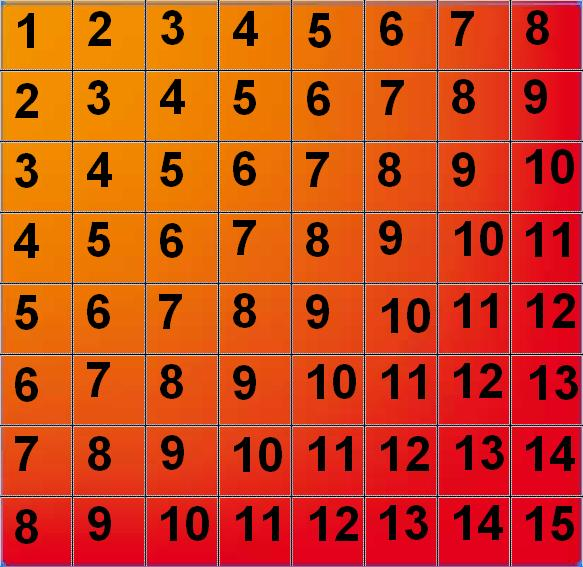
\includegraphics[scale=0.25]{refuerzos.jpg}
  \caption{Refuerzos para un tablero de 8 por 8 con salida en (7,7).}
	\end{figure}	
	La motivaci\'on de este refuerzo es que el agente trate de dirigirse hacia la salida.
	\end{itemize}

\item[\texttt{BOMB\_REWARD\_POLICY}] Rewards por destruir paredes.
	\begin{itemize}
	\item \texttt{BOMB\_NO\_REWARD}: No se agrega refuerzos intermedios adicionales.
	\item \texttt{BOMB\_REWARD\_PER\_STONE\_DESTROYED}: Cada vez que el agente destruye una pared, sin morir, recibe un refuerzo igual al \texttt{BOMB\_REWARD} del archivo de settings. La idea de este refuerzo es que el agente aprenda que debe destruir paredes.
	\item \texttt{BOMB\_REWARD\_PER\_STONE\_DESTROYED\_PROPORTIONAL\_TO\_EXIT}: el refuerzo anterior, usado solo podr\'ia hacer que el agente, por lo menos en las primeras iteraciones, intente romper muchas paredes. Por eso agregamos esta opci\'on, que le da mayor valor a romper paredes cercanas a la salida. La formula para este valor es $bomb\_reward \times cercania\_a\_la\_salida$ calculando la cercan\'ia de la misma forma que antes.
	\end{itemize}

	
\item[\texttt{NO\_ACTION\_NEGATIVE\_REWARD}] Para desalentar el que el agente realizara acciones que no modificaran el estado, agregamos este booleano. Si se activa, cada vez que el agente realiza una acci\'on sin efecto, se le da un refuerzo negativo. Por defecto, cada vez que el agente realice una acci\'on que no cambie el estado, se le dar\'a un refuerzo negativo de -10.

\item[\texttt{INITIAL\_REWARD}] En la misma l\'inea que el \'item anterior, tambi\'en permitimos variar el refuerzo que se le da al agente al realizar cualquier acci\'on. La idea es que si este valor fuera negativo, el agente intentar\'a llegar lo mas r\'apido a la salida. Esta idea se integra al $\gamma$, pero permite explicitar el valor negativo de realizar acciones. Por defecto, el agente recibe un -1 por cada acci\'on realizada.

\end{description}

	Las funciones para la aplicaci\'on de estos refuerzos se pueden encontrar en el archivo \textit{Rewards.py} y son llamadas desde Task de acuerdo a las pol\'iticas elegidas por el usuario en el archivo de Settings.
 
\section{Pruebas y resultados}
	\subsection{Sin Rewards Intermedios}


	\subsection{Aplicando Rewards Intermedios}
	
A continuaci\'on evaluamos cada uno de los distintos algoritmos aplicando las distintas configuraciones de rewards intermedios antes mencionadas, tanto para navegaci\'on como para stones destruidas. El objetivo es analizar c\'omo la aplicaci\'on de recompensas intermedias favorecen, a modo de breadcrumb, la convergencia de los distintos agentes\footnote{No incluimos a los agentes de R-Max factorizado ni Sarsa-$\lambda$ pues los resultados obtenidos no fueron satisfactorios, independientemente de la aplicaci\'on de rewards}.

Todas las pruebas fueron ejecutadas sobre tableros de $5 \times 5$, a excepci\'on de RMax que fue ejecutado sobre un tablero de $3 \times 3$ debido al alto tiempo de procesamiento que tuvo.

\subsubsection{Q-Learning}

En la figura \ref{fig:qlearnrewards} presentamos el comportamiento del algoritmo de q-learning de acuerdo a las distintas configuraciones de rewards. 

Como se puede observar, la aplicaci\'on de navigation rewards no genera una mejora importante sobre el punto de convergencia (por el contrario, lo empeora), aunque s\'i ayuda a que las partidas ganadas se mantengan m\'as cercanas al \'optimo. Resulta particular el hecho de que los juegos realizados previos al punto de convergencia requieran una mayor cantidad de movimientos al aplicar estas rewards.

Las bomb rewards, por otro lado, tienen un efecto importante en el momento en que el algoritmo converge, reduciendo notablemente la cantidad de juegos que el agente necesita para llegar a una estrategia ganadora, as\'i como la cantidad de movimientos usados en los juegos iniciales. La diferencia entre las dos configuraciones de bomb rewards es \'infima.

\begin{figure}
\centering
\subfloat[Sin rewards intermedias]{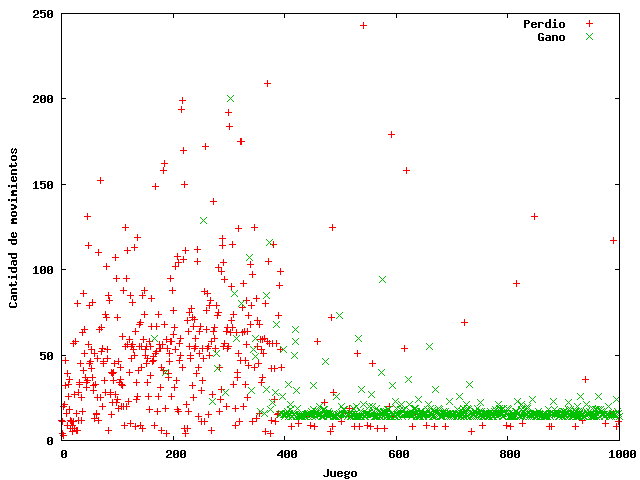
\includegraphics[width=0.5\textwidth]{corridas/QlearningNoRewards-result.png}}
\subfloat[Navigation rewards]{\label{fig:tiger}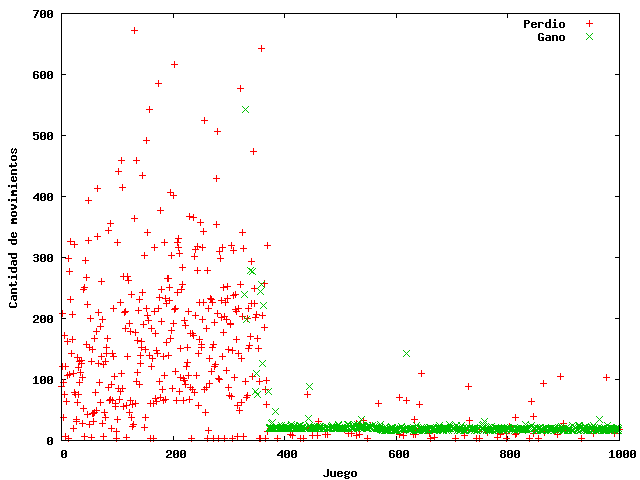
\includegraphics[width=0.5\textwidth]{corridas/QlearningNavigationReward-result.png}}
\\
\subfloat[Bomb rewards]{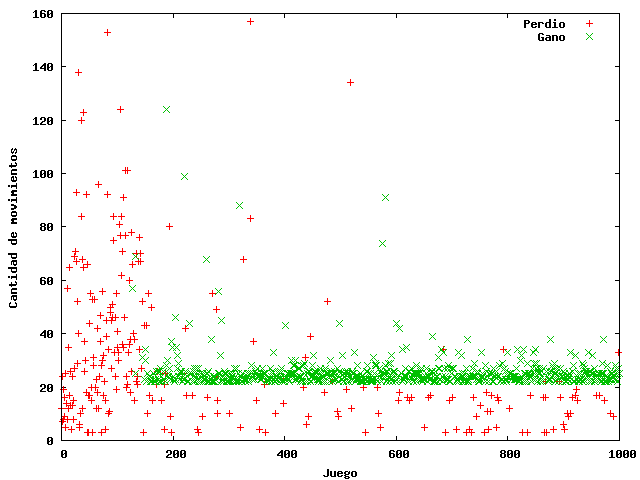
\includegraphics[width=0.5\textwidth]{corridas/Qlearning-bombR-result.png}}
\subfloat[Bomb rewards relativas a la distancia a la salida]{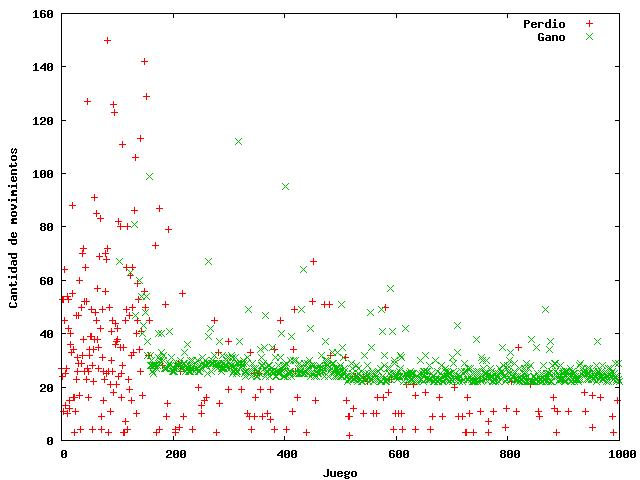
\includegraphics[width=0.5\textwidth]{corridas/QLearningBombProportionalToExit-result.png}}
\caption{Comportamiento del algoritmo q-learning dependiendo de las distintas configuraciones de rewards intermedias; cada gr\'afico muestra la cantidad de movimientos en funci\'on del n\'umero de juego, distinguiendo si el agente gan\'o o perdi\'o.}
\label{fig:qlearnrewards}
\end{figure}


\subsubsection{Dyna}

En \ref{fig:dynarew} presentamos los gr\'aficos correspondientes al efecto de la aplicaci\'on de rewards intermedias para el algoritmo dyna.

En este caso, a diferencia de q-learning, la aplicaci\'on de rewards intermedias para navegaci\'on mejor\'o notablemente la velocidad de convergencia del algoritmo, al punto de que el agente perdiera en muy pocas oportunidades, dando excelentes resultados. De todas maneras, y al igual que en el caso de q-learning, la aplicaci\'on de estas rewards llev\'o a que en los juegos perdidos la cantidad de movimientos fuera mucho mayor.

Las bomb rewards, por otra parte, tambi\'en mejoraron notablemente la velocidad de convergencia hacia una estrategia ganadora, aunque en menor medida que las rewards de navegaci\'on. Nuevamente se observa una reducci\'on en la cantidad de movimientos realizada en los juegos perdidos. 

En este caso, las recompensas constantes para todas las stones dieron resultados levemente mejores que la contraparte proporcional a la distancia a la salida.

\begin{figure}
\centering
\subfloat[Sin rewards intermedias]{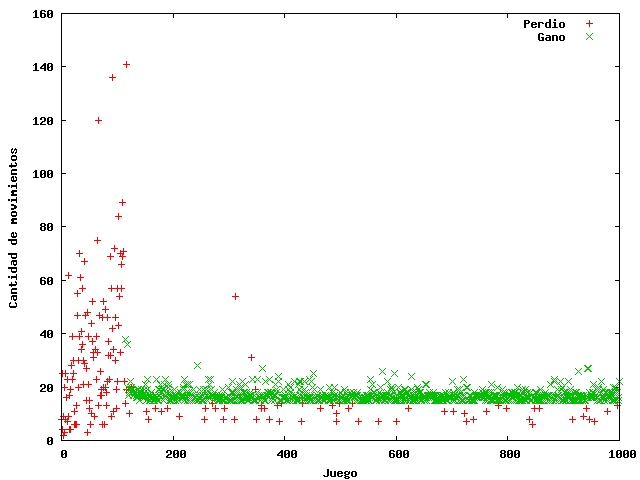
\includegraphics[width=0.5\textwidth]{corridas/DynaNoRewards-result.png}}
\subfloat[Navigation rewards]{\label{fig:tiger}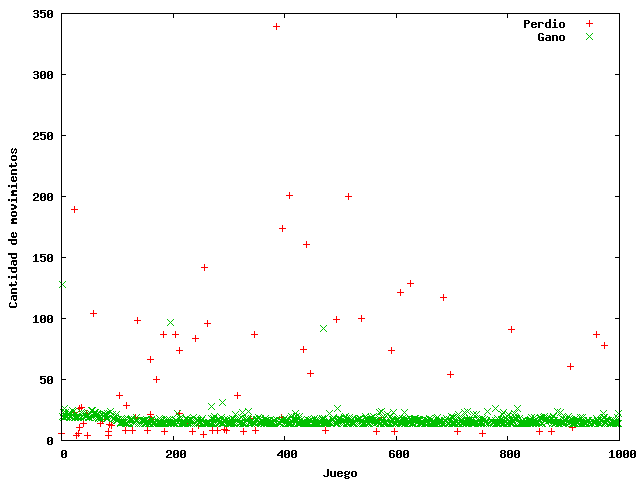
\includegraphics[width=0.5\textwidth]{corridas/DynaNavigationRewards-result.png}}
\\
\subfloat[Bomb rewards]{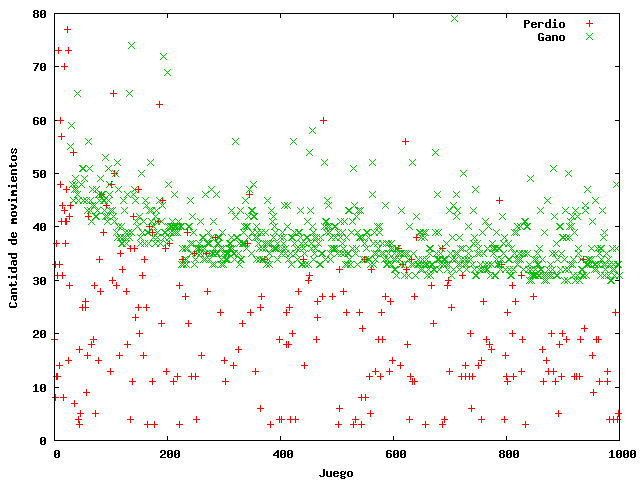
\includegraphics[width=0.5\textwidth]{corridas/DynaBombRewards-result.png}}
\subfloat[Bomb rewards relativas a la distancia a la salida]{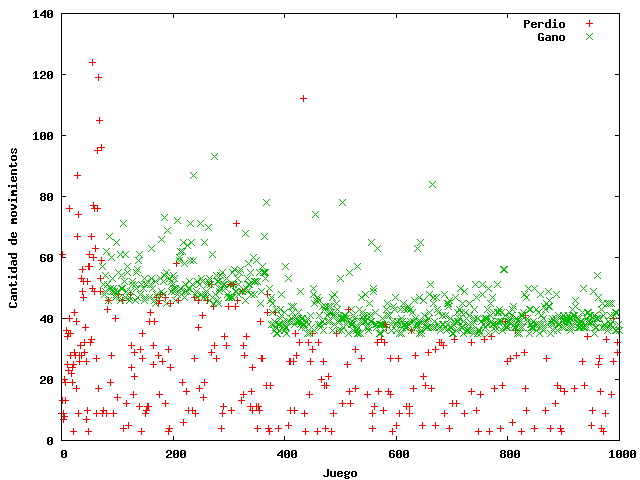
\includegraphics[width=0.5\textwidth]{corridas/DynaBombProportionalToExit-result.png}}
\caption{Comportamiento del algoritmo dyna dependiendo de las distintas configuraciones de rewards intermedias; cada gr\'afico muestra la cantidad de movimientos en funci\'on del n\'umero de juego, distinguiendo si el agente gan\'o o perdi\'o.}
\label{fig:dynarew}
\end{figure}

\subsubsection{R-Max}

Para el caso de R-Max, como puede verse en la figura \ref{fig:rmaxrew}, el comportamiento var\'ia muy poco de acuerdo a las rewards aplicadas. En todos los casos se mantiene el comportamiento de arribar a una estrategia ganadora r\'apidamente y no intentar explorar alternativa alguna. 

Las ligeras diferencias observadas entre las distintas configuraciones de rewards dependen m\'as del componente aleatorio que tiene el algoritmo a la hora de elegir una acci\'on (en caso de no tener informaci\'on suficiente para tomar una decisi\'on), que de una diferencia efectiva generada por las rewards intermedias.

De todas maneras, cabe destacar que la estrategia arribada pasa de tener $10$ movimientos en los casos sin rewards y con rewards constantes por stones, a tener $9$ en las configuraciones restantes.

\begin{figure}
\centering
\subfloat[Sin rewards intermedias]{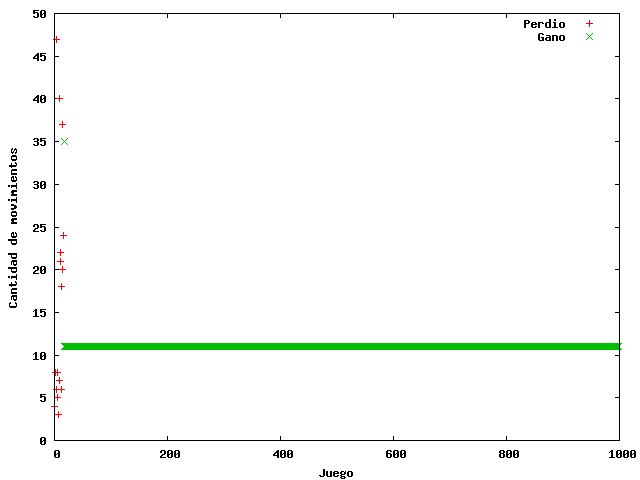
\includegraphics[width=0.5\textwidth]{corridas/RmaxNoRewards-result.png}}
\subfloat[Navigation rewards]{\label{fig:tiger}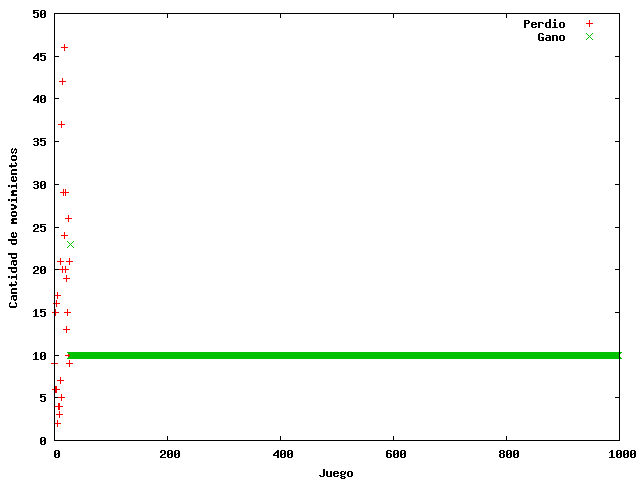
\includegraphics[width=0.5\textwidth]{corridas/RMaxNavigationRewards-result.png}}
\\
\subfloat[Bomb rewards]{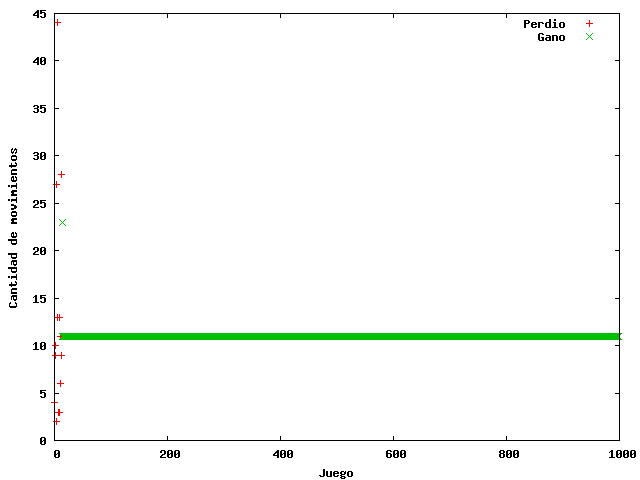
\includegraphics[width=0.5\textwidth]{corridas/RMaxBombRewards-result.png}}
\subfloat[Bomb rewards relativas a la distancia a la salida]{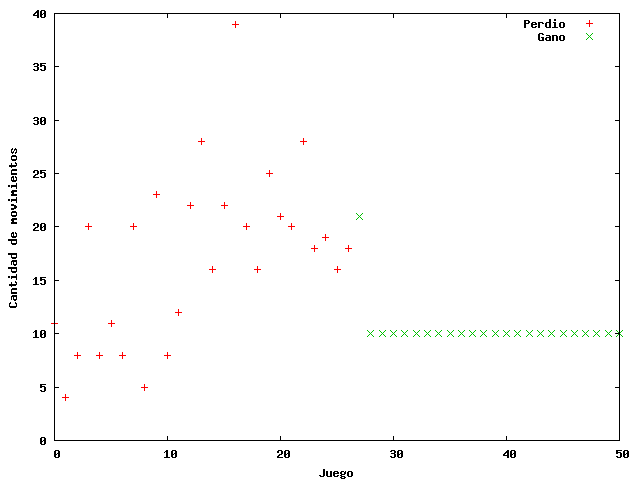
\includegraphics[width=0.5\textwidth]{corridas/RMaxBombProportionalToExit-result.png}}
\caption{Comportamiento del algoritmo R-Max dependiendo de las distintas configuraciones de rewards intermedias; cada gr\'afico muestra la cantidad de movimientos en funci\'on del n\'umero de juego, distinguiendo si el agente gan\'o o perdi\'o.}
\label{fig:rmaxrew}
\end{figure}

\subsubsection{Sarsa}

Los resultados de las aplicaciones de las rewards intermedios para Sarsa pueden verse en la figura \ref{fig:sarsarew}. Si bien los resultados obtenidos por Sarsa, independientemente de las rewards, no son muy satisfactorios, tanto por la cantidad de juegos perdidos como por la cantidad de movimientos por juego, el uso rewards muestra una cierta mejora en la cantidad de juegos ganados.

Las bomb rewards, al igual que en los casos anteriores, generan una leve reducci\'on en la cantidad de movimientos por juego, aunque en este caso afectando tanto a los juegos ganados como a los perdidos.

\begin{figure}
\centering
\subfloat[Sin rewards intermedias]{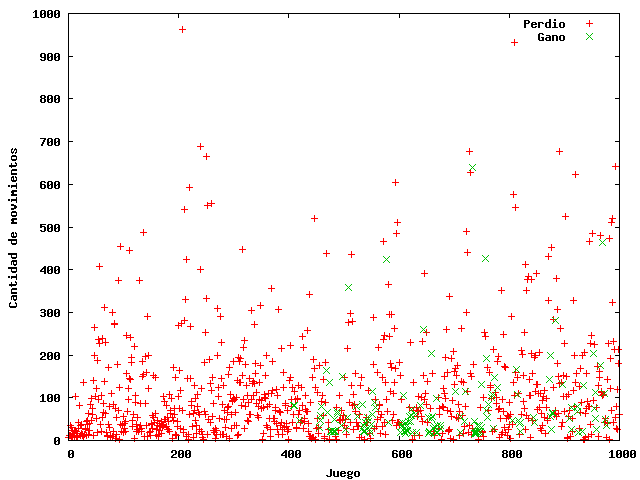
\includegraphics[width=0.5\textwidth]{corridas/SarsaNoRewards-result.png}}
\subfloat[Navigation rewards]{\label{fig:tiger}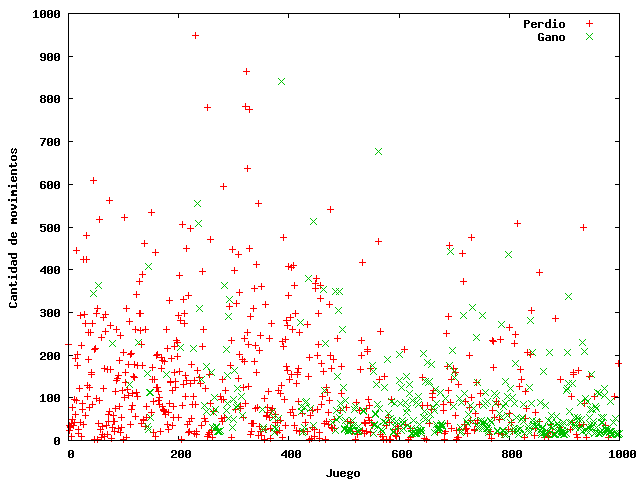
\includegraphics[width=0.5\textwidth]{corridas/SarsaNavigationReward-result.png}}
\\
\subfloat[Bomb rewards]{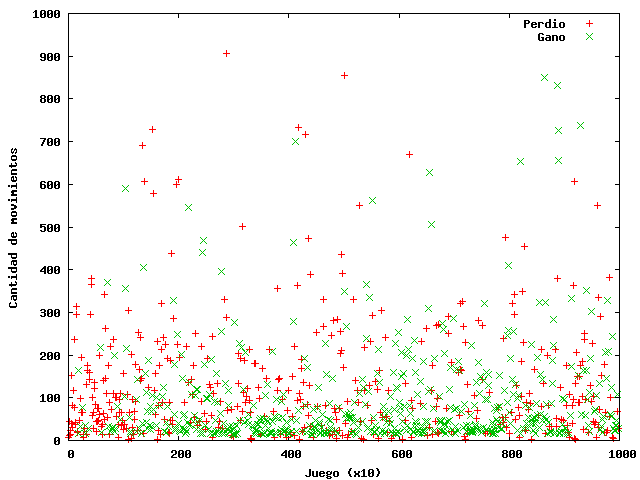
\includegraphics[width=0.5\textwidth]{corridas/SarsaBombReward-result.png}}
\subfloat[Bomb rewards relativas a la distancia a la salida]{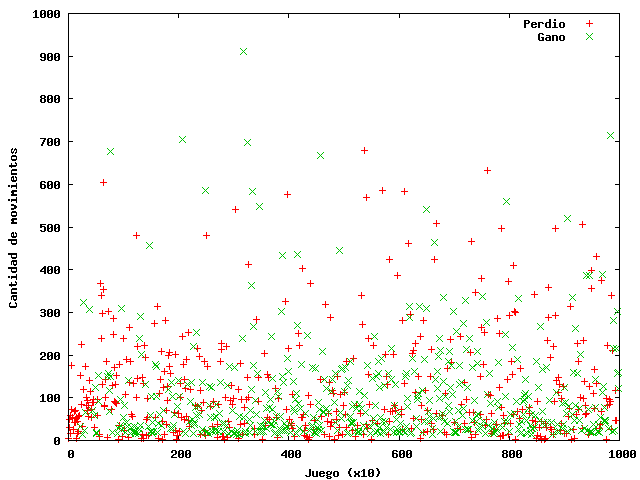
\includegraphics[width=0.5\textwidth]{corridas/SarsaBombProportionalToExit-result.png}}
\caption{Comportamiento del algoritmo Sarsa dependiendo de las distintas configuraciones de rewards intermedias; cada gr\'afico muestra la cantidad de movimientos en funci\'on del n\'umero de juego (notar que el n\'umero de juego debe multiplicarse por 10), distinguiendo si el agente gan\'o o perdi\'o.}
\label{fig:sarsarew}
\end{figure}


\clearpage


\subsection{Comparaci\'on}

Volcamos en la tabla \ref{table:rewards} los datos correspondientes al tiempo promedio por movimiento, el punto de convergencia y la menor cantidad de movimientos alcanzada por cada algoritmo seg\'un distintas rewards para una f\'acil comparaci\'on entre ellos. Es importante para la comparaci\'on recordar que RMax fue ejecutado sobre un tablero de menor tama\'no; asimismo incluimos en esta secci\'on Sarsa-$\lambda$ pese a no haber logrado resultados aceptables.

Los tiempos de procesamiento se ven poco afectados por la aplicaci\'on de rewards, manteni\'endose bajos para algoritmos livianos como Q-learning o Sarsa, y con valores m\'as altos para Dyna, Sarsa-$\lambda$ y especialmente RMax.

La convergencia var\'ia dependiendo del algoritmo. Un model-based, como ser Dyna, acelera notablemente la convergencia al tener hints de navegaci\'on o de bombas, aunque la aplicaci\'on de rewards proporcionales a la salida para las bombas result\'o no ser acertada. En el caso de Q-learning, siendo model free, por el contrario, las rewards por bombas aceleran la convergencia, mientras que la navegaci\'on la hace m\'as lenta.

Tal vez la conclusi\'on m\'as destacable sea el cambio generado en la estrategia \'optima al a\'nadir rewards por stones destruidas. Los algoritmos que mejores resultados dieron, Q-Learning y Dyna, generan una estrategia sub\'optima al incluir estas rewards. Esto puede explicarse en el hecho de que el agente, al obtener una recompensa al destruir una pared, opta por destruir paredes innecesarias en lugar de dirigirse a la salida lo m\'as r\'apidamente posible. 

De este hecho concluimos que el decay factor $\gamma$ no era lo suficientemente pronunciado, con lo que en t\'erminos de largo plazo el agente juzg\'o que era m\'as provechoso destruir m\'as stones a pesar de ver reducida por decay la recompensa final.

\begin{table}
\label{table:rewards}
\centering

\begin{tabular}{|ll|r|r|r|}
\hline
\textbf{Agente} & \textbf{Reward} & \textbf{Tiempo} & \textbf{Convergencia} & \textbf{Optimo} \\
\hline
\hline
Q Learning & None & 7.41e-05 & 167 & 13 \\
Q Learning & Navigation & 6.45e-05 & 329 & 13 \\
Q Learning & Bomb & 7.34e-05 & 129 & 21 \\
Q Learning & $\Delta_{exit}$ Bomb & 7.69e-05 & 105 & 21 \\
\hline
Dyna & None & 1.27e-02 & 115 & 13 \\
Dyna & Navigation & 1.19e-03 & 2 & 13 \\
Dyna & Bomb & 8.79e-03 & 30 & 27 \\
Dyna & $\Delta_{exit}$ Bomb & 3.40e-03 & 155 & 24 \\
\hline
Sarsa & None & 5.89e-05 & None & 13 \\
Sarsa & Navigation & 4.77e-05 & None & 13 \\
Sarsa & Bomb& 6.04e-05 & None & 13 \\
Sarsa & $\Delta_{exit}$ Bomb & 5.26e-05 & None & 13 \\
\hline
Sarsa-$\lambda$ & None & 1.89e-02 & None & 16 \\
Sarsa-$\lambda$ & Bomb & 1.89e-02 & None & 26 \\
Sarsa-$\lambda$ & Navigation & 1.77e-02 & None & 20 \\
Sarsa-$\lambda$ & $\Delta_{exit}$ Bomb & 1.61e-02 & None & 23 \\
\hline
R-Max $_{3 \times 3}$ & None & 6.15e-02 & 18 & 10 \\
R-Max $_{3 \times 3}$& Navigation & 1.08e-01 & 29 & 9 \\
R-Max $_{3 \times 3}$& Bomb & 2.73e-02 & 15 & 10 \\
R-Max $_{3 \times 3}$& $\Delta_{exit}$ Bomb & 1.14e-01 & 28 & 9 \\
\hline
\end{tabular}

\caption{Tiempo promedio por movimiento, cantidad de juegos requerida hasta lograr convergencia y mejor estrategia desarrollada para ganar medida en cantidad de movimientos; definimos convergencia como el punto a partir del cual la cantidad de juegos perdidos no supera determinado porcentaje ($20\%$) de los ganados.}

\end{table}


\clearpage




	\subsection{Rewards Intermedios por posici\'on del bomberman}
	\subsection{Rewards Intermedios por explotar bomba}
	\subsection{Rewards Intermedios por explotar bomba relativo a la posicion de la bomba}

\section{Stats}

\begin{table}
\centering

\begin{tabular}{|l|r|r|r|}
\hline
\textbf{Agente} & \textbf{Tiempo} & \textbf{Convergencia} & \textbf{Optimo} \\
\hline
DynaBombRewards-result.out & 8.79e-03 & 30 & 27 \\
Qlearning-bombR-result.out & 7.34e-05 & 129 & 21 \\
SarsaBombReward-result.out & 6.04e-05 & None & 13 \\
SarsaLambdaBombRewards-result.out & 1.89e-02 & None & 26 \\
DynaBombProportionalToExit-result.out & 3.40e-03 & 155 & 24 \\
QLearningBombProportionalToExit-result.out & 7.69e-05 & 105 & 21 \\
SarsaBombProportionalToExit-result.out & 5.26e-05 & None & 13 \\
SarsaLambdaBombProportionalToExit-result.out & 1.61e-02 & None & 23 \\
DynaNavigationRewards-result.out & 1.19e-03 & 2 & 13 \\
QlearningNavigationReward-result.out & 6.45e-05 & 329 & 13 \\
SarsaLambdaNavigationRewards-result.out & 1.77e-02 & None & 20 \\
SarsaNavigationReward-result.out & 4.77e-05 & None & 13 \\
DynaNoRewards-result.out & 1.27e-02 & 115 & 13 \\
QlearningNoRewards-result.out & 7.41e-05 & 167 & 13 \\
SarsaLambdaNoRewards-result.out & 1.89e-02 & None & 16 \\
SarsaNoRewards-result.out & 5.89e-05 & None & 13 \\
RMaxBombProportionalToExit-result.out & 1.14e-01 & 28 & 9 \\
RMaxBombRewards-result.out & 2.73e-02 & 15 & 10 \\
RMaxNavigationRewards-result.out & 1.08e-01 & 29 & 9 \\
RmaxNoRewards-result.out & 6.15e-02 & 18 & 10 \\
StochasticExplo.Dyna-result.out & 4.26e-03 & 19 & 16 \\
StochasticExplo.QLearn-result.out & 5.01e-05 & 8 & 13 \\
StochasticExplo.Sarsa-result.out & 4.18e-05 & 4997 & 17 \\
StochasticNav.Dyna-result.out & 3.46e-03 & 4962 & 14 \\
StochasticNav.QLearn-result.out & 5.74e-05 & 372 & 13 \\
StochasticNav.Sarsa-result.out & 4.47e-05 & None & 13 \\
\end{tabular}

\caption{Tiempo promedio por movimiento, cantidad de juegos requerida hasta lograr convergencia y mejor estrategia desarrollada para ganar medida en cantidad de movimientos; definimos convergencia como el punto a partir del cual la cantidad de juegos perdidos no supera determinado porcentaje ($20\%$) de los ganados.}

\end{table}

\section{Conclusiones}

\clearpage

\begin{thebibliography}{widest-label}

\bibitem{li} Lihong Li: \textit{A unifying framework for computational reinforcement learning theory}, \texttt{http://www.research.rutgers.edu/~lihong/pub/Li09Unifying.pdf}

\bibitem{rmax} Ronen I. Brafman, Moshe Tennenholtz: \textit{R-max A General Polynomial Time Algorithm for
Near-Optimal Reinforcement Learning}

\bibitem{rmaxfact} Carlos Guestrin, Relu Patrascu, Dale Schuurmans: \textit{Algorithm-Directed Exploration for Model-Based Reinforcement Learning in Factored MDPs}

\bibitem{kroonicmla09} Mark Kroon, Shimon Whiteson: \textit{Automatic Feature Selection for Model-Based Reinforcement Learning in Factored MDPs}

\bibitem{dbne3} Michael Kearns, Daphne Koller: \textit{Efficient Reinforcement Learning in Factored MDPs}

\bibitem{AAAI07-102} Alexander L. Strehl, Carlos Diuk, Michael L. Littman: \textit{Efficient Structure Learning in Factored-state MDPs}

\bibitem{12-64-FP-0295} Todd Hester, Peter Stone: \textit{Generalized Model Learning for Reinforcement Learning in Factored Domains}

\bibitem{05-Broo87} Carlos Diuk, Lihong Li, Bethany R. Leffler: \textit{The Adaptive k-Meteorologists Problem and Its Application to Structure Learning and Feature Selection in Reinforcement Learning}

\bibitem{c-refuerzo} Eduardo Morales, Jesus Gonzalez: \textit{Aprendizaje Computacional, Cap\'itulo 11: Aprendizaje por Refuerzo}, \texttt{http://ccc.inaoep.mx/~jagonzalez/ML/c-refuerzo.pdf}

\bibitem{pacrl} Alexander L. Strehl, Lihong Li, Eric Wiewiora, John Langford, Michael L. Littman: \textit{PAC Model-Free Reinforcement Learning}, \texttt{http://hunch.net/~jl/projects/RL/Delayed\_Q/icml-talk.pdf}

\end{thebibliography}
	
\end{document}